\documentclass[border=4pt]{standalone}
\usepackage{amsmath,amssymb}
\usepackage{tikz}
\usetikzlibrary{arrows.meta,decorations.pathreplacing,patterns,calc,positioning,shapes.geometric}
\usepackage{pgfplots}
\pgfplotsset{compat=newest}
\begin{document}
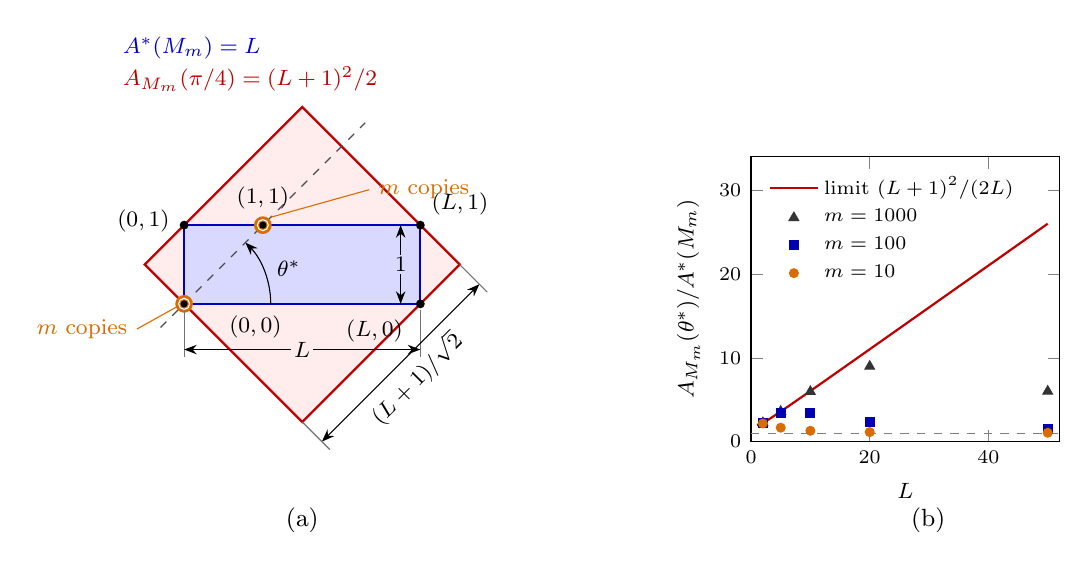
\begin{tikzpicture}[>={Stealth[length=1.6mm]},
  lab/.style={font=\footnotesize},
  dim/.style={<->,thin},
  ext/.style={thin,black!55}]
%======================== (a) the multiset M_m for L = 3 and the two rectangles
\begin{scope}[scale=1.0]
  % rectangle of area A_M(pi/4) = (L+1)^2/2 = 8, sides (L+1)/sqrt(2)
  \fill[red!7] (1.5,-1.5) -- (3.5,0.5) -- (1.5,2.5) -- (-0.5,0.5) -- cycle;
  \draw[red!75!black,thick] (1.5,-1.5) -- (3.5,0.5) -- (1.5,2.5) -- (-0.5,0.5) -- cycle;
  % minimum-area rectangle [0,L]x[0,1], area L = 3
  \fill[blue!15] (0,0) rectangle (3,1);
  \draw[blue!75!black,thick] (0,0) rectangle (3,1);
  % principal axis of the limiting two-point distribution
  \draw[black!70,dashed] (-0.3,-0.3) -- (2.3,2.3);
  \draw[->,thin] (1.1,0) arc[start angle=0,end angle=45,radius=1.1];
  \node[lab] at (1.33,0.45) {$\theta^*$};
  % points of M_m
  \foreach \p in {(3,0),(3,1),(0,1)} \fill \p circle (1.6pt);
  \foreach \p in {(0,0),(1,1)} {\fill[orange!85!black] \p circle (3.2pt); \draw[white,thin] \p circle (2.0pt); \fill \p circle (1.3pt);}
  \node[lab,anchor=north west] at (0.45,-0.03) {$(0,0)$};
  \node[lab,anchor=north east] at (2.9,-0.08) {$(L,0)$};
  \node[lab,anchor=south west] at (3.02,1) {$(L,1)$};
  \node[lab,anchor=east] at (-0.06,1.05) {$(0,1)$};
  \node[lab,anchor=south] at (1.0,1.08) {$(1,1)$};
  \draw[ext,orange!85!black] (-0.08,-0.03) -- (-0.6,-0.32) node[lab,anchor=east] {$m$ copies};
  \draw[ext,orange!85!black] (1.1,1.1) -- (2.35,1.45) node[lab,anchor=west] {$m$ copies};
  % dimensions of the minimum-area rectangle
  \draw[ext] (0,-0.08) -- (0,-0.68); \draw[ext] (3,-0.08) -- (3,-0.68);
  \draw[dim] (0,-0.58) -- node[lab,fill=red!7,inner sep=1pt] {$L$} (3,-0.58);
  \draw[dim] (2.75,0) -- node[lab,fill=blue!15,inner sep=1pt] {$1$} (2.75,1);
  % sides of the rectangle at pi/4
  \draw[dim] ($(1.5,-1.5)+(0.25,-0.25)$) -- node[lab,sloped,below] {$(L+1)/\sqrt{2}$} ($(3.5,0.5)+(0.25,-0.25)$);
  \draw[ext] (1.5,-1.5) -- ++(0.35,-0.35); \draw[ext] (3.5,0.5) -- ++(0.35,-0.35);
  \node[lab,blue!75!black,anchor=west] at (-0.9,3.25) {$A^*(M_m)=L$};
  \node[lab,red!75!black,anchor=west] at (-0.9,2.85) {$A_{M_m}(\pi/4)=(L+1)^2/2$};
  \node[font=\small] at (1.5,-2.75) {(a)};
\end{scope}
%======================== (b) ratio as a function of L
\begin{scope}[xshift=7.2cm,yshift=-1.75cm]
\begin{axis}[width=5.5cm,height=5.2cm,
  xmin=0,xmax=52,ymin=0,ymax=34,
  xlabel={$L$},ylabel={$A_{M_m}(\theta^*)/A^*(M_m)$},
  label style={font=\footnotesize},tick label style={font=\scriptsize},
  legend style={font=\scriptsize,at={(0.03,0.97)},anchor=north west,draw=none,fill=none},
  legend cell align=left]
  \addplot[red!75!black,thick,domain=1:50,samples=100] {(x+1)^2/(2*x)};
  \addlegendentry{limit $(L+1)^2/(2L)$}
  \addplot[only marks,mark=triangle*,mark size=2pt,black!80] coordinates {(2,2.25) (5,3.60) (10,5.97) (20,8.98) (50,6.01)};
  \addlegendentry{$m=1000$}
  \addplot[only marks,mark=square*,mark size=1.6pt,blue!70!black] coordinates {(2,2.25) (5,3.42) (10,3.47) (20,2.32) (50,1.52)};
  \addlegendentry{$m=100$}
  \addplot[only marks,mark=*,mark size=1.6pt,orange!85!black] coordinates {(2,2.17) (5,1.67) (10,1.30) (20,1.14) (50,1.06)};
  \addlegendentry{$m=10$}
  \addplot[black!50,dashed,domain=0:52] {1};
\end{axis}
\node[font=\small] at (2.25,-1.0) {(b)};
\end{scope}
\end{tikzpicture}
\end{document}
